\documentclass{ximera}

%\usepackage{todonotes}

\newcommand{\todo}{}

\usepackage{tkz-euclide}
\tikzset{>=stealth} %% cool arrow head
\tikzset{shorten <>/.style={ shorten >=#1, shorten <=#1 } } %% allows shorter vectors

\usepackage{tkz-tab}  %% sign charts
\usetikzlibrary{decorations.pathreplacing} 

\usetikzlibrary{backgrounds} %% for boxes around graphs
\usetikzlibrary{shapes,positioning}  %% Clouds and stars
\usetikzlibrary{matrix} %% for matrix
\usepgfplotslibrary{polar} %% for polar plots
\usetkzobj{all}
\usepackage[makeroom]{cancel} %% for strike outs
%\usepackage{mathtools} %% for pretty underbrace % Breaks Ximera
\usepackage{multicol}

\usepackage{polynom}



\usepackage[many]{tcolorbox}  %% for titled boxes
\newtcolorbox{xbox}[1]{%
    tikznode boxed title,
    enhanced,
    arc=0mm,
    interior style={white},
    attach boxed title to top center= {yshift=-\tcboxedtitleheight/2},
    fonttitle=\bfseries,
    colbacktitle=white,coltitle=black,
    boxed title style={size=normal,colframe=white,boxrule=0pt},
    title={#1}}


\usepackage{array}
\setlength{\extrarowheight}{+.1cm}   
\newdimen\digitwidth
\settowidth\digitwidth{9}
\def\divrule#1#2{
\noalign{\moveright#1\digitwidth
\vbox{\hrule width#2\digitwidth}}}





\newcommand{\RR}{\mathbb R}
\newcommand{\R}{\mathbb R}
\newcommand{\N}{\mathbb N}
\newcommand{\Z}{\mathbb Z}

%\renewcommand{\d}{\,d\!}
\renewcommand{\d}{\mathop{}\!d}
\newcommand{\dd}[2][]{\frac{\d #1}{\d #2}}
\newcommand{\pp}[2][]{\frac{\partial #1}{\partial #2}}
\renewcommand{\l}{\ell}
\newcommand{\ddx}{\frac{d}{\d x}}
\newcommand{\ddt}{\frac{d}{\d t}}

\newcommand{\zeroOverZero}{\ensuremath{\boldsymbol{\tfrac{0}{0}}}}
\newcommand{\inftyOverInfty}{\ensuremath{\boldsymbol{\tfrac{\infty}{\infty}}}}
\newcommand{\zeroOverInfty}{\ensuremath{\boldsymbol{\tfrac{0}{\infty}}}}
\newcommand{\zeroTimesInfty}{\ensuremath{\small\boldsymbol{0\cdot \infty}}}
\newcommand{\inftyMinusInfty}{\ensuremath{\small\boldsymbol{\infty - \infty}}}
\newcommand{\oneToInfty}{\ensuremath{\boldsymbol{1^\infty}}}
\newcommand{\zeroToZero}{\ensuremath{\boldsymbol{0^0}}}
\newcommand{\inftyToZero}{\ensuremath{\boldsymbol{\infty^0}}}



\newcommand{\numOverZero}{\ensuremath{\boldsymbol{\tfrac{\#}{0}}}}
\newcommand{\dfn}{\textbf}
%\newcommand{\unit}{\,\mathrm}
\newcommand{\unit}{\mathop{}\!\mathrm}
\newcommand{\eval}[1]{\bigg[ #1 \bigg]}
\newcommand{\seq}[1]{\left( #1 \right)}
\renewcommand{\epsilon}{\varepsilon}
\renewcommand{\iff}{\Leftrightarrow}

\DeclareMathOperator{\arccot}{arccot}
\DeclareMathOperator{\arcsec}{arcsec}
\DeclareMathOperator{\arccsc}{arccsc}
\DeclareMathOperator{\si}{Si}
\DeclareMathOperator{\proj}{proj}
\DeclareMathOperator{\scal}{scal}


\newcommand{\tightoverset}[2]{% for arrow vec
  \mathop{#2}\limits^{\vbox to -.5ex{\kern-0.75ex\hbox{$#1$}\vss}}}
\newcommand{\arrowvec}[1]{\tightoverset{\scriptstyle\rightharpoonup}{#1}}
\renewcommand{\vec}{\mathbf}
\newcommand{\veci}{\vec{i}}
\newcommand{\vecj}{\vec{j}}
\newcommand{\veck}{\vec{k}}
\newcommand{\vecl}{\boldsymbol{\l}}

\newcommand{\dotp}{\bullet}
\newcommand{\cross}{\boldsymbol\times}
\newcommand{\grad}{\boldsymbol\nabla}
\newcommand{\divergence}{\grad\dotp}
\newcommand{\curl}{\grad\cross}
%\DeclareMathOperator{\divergence}{divergence}
%\DeclareMathOperator{\curl}[1]{\grad\cross #1}


\colorlet{textColor}{black} 
\colorlet{background}{white}
\colorlet{penColor}{blue!50!black} % Color of a curve in a plot
\colorlet{penColor2}{red!50!black}% Color of a curve in a plot
\colorlet{penColor3}{red!50!blue} % Color of a curve in a plot
\colorlet{penColor4}{green!50!black} % Color of a curve in a plot
\colorlet{penColor5}{orange!80!black} % Color of a curve in a plot
\colorlet{fill1}{penColor!20} % Color of fill in a plot
\colorlet{fill2}{penColor2!20} % Color of fill in a plot
\colorlet{fillp}{fill1} % Color of positive area
\colorlet{filln}{penColor2!20} % Color of negative area
\colorlet{fill3}{penColor3!20} % Fill
\colorlet{fill4}{penColor4!20} % Fill
\colorlet{fill5}{penColor5!20} % Fill
\colorlet{gridColor}{gray!50} % Color of grid in a plot

\newcommand{\surfaceColor}{violet}
\newcommand{\surfaceColorTwo}{redyellow}
\newcommand{\sliceColor}{greenyellow}




\pgfmathdeclarefunction{gauss}{2}{% gives gaussian
  \pgfmathparse{1/(#2*sqrt(2*pi))*exp(-((x-#1)^2)/(2*#2^2))}%
}


%%%%%%%%%%%%%
%% Vectors
%%%%%%%%%%%%%

%% Simple horiz vectors
\renewcommand{\vector}[1]{\left\langle #1\right\rangle}


%% %% Complex Horiz Vectors with angle brackets
%% \makeatletter
%% \renewcommand{\vector}[2][ , ]{\left\langle%
%%   \def\nextitem{\def\nextitem{#1}}%
%%   \@for \el:=#2\do{\nextitem\el}\right\rangle%
%% }
%% \makeatother

%% %% Vertical Vectors
%% \def\vector#1{\begin{bmatrix}\vecListA#1,,\end{bmatrix}}
%% \def\vecListA#1,{\if,#1,\else #1\cr \expandafter \vecListA \fi}

%%%%%%%%%%%%%
%% End of vectors
%%%%%%%%%%%%%

%\newcommand{\fullwidth}{}
%\newcommand{\normalwidth}{}



%% makes a snazzy t-chart for evaluating functions
%\newenvironment{tchart}{\rowcolors{2}{}{background!90!textColor}\array}{\endarray}

%%This is to help with formatting on future title pages.
\newenvironment{sectionOutcomes}{}{} 



%% Flowchart stuff
%\tikzstyle{startstop} = [rectangle, rounded corners, minimum width=3cm, minimum height=1cm,text centered, draw=black]
%\tikzstyle{question} = [rectangle, minimum width=3cm, minimum height=1cm, text centered, draw=black]
%\tikzstyle{decision} = [trapezium, trapezium left angle=70, trapezium right angle=110, minimum width=3cm, minimum height=1cm, text centered, draw=black]
%\tikzstyle{question} = [rectangle, rounded corners, minimum width=3cm, minimum height=1cm,text centered, draw=black]
%\tikzstyle{process} = [rectangle, minimum width=3cm, minimum height=1cm, text centered, draw=black]
%\tikzstyle{decision} = [trapezium, trapezium left angle=70, trapezium right angle=110, minimum width=3cm, minimum height=1cm, text centered, draw=black]


\outcome{Identify word problems as related rates problems.}
\outcome{Solve related rates word problems.}
\outcome{Translate word problems into mathematical expressions.}

\title[Dig-In:]{Applied related rates}

\begin{document}
\begin{abstract}
  We solve related rates problems in context.
\end{abstract}
\maketitle

Now we are ready to solve related rates problems in context. Just as
before, we are going to follow essentially the same plan of attack in
each problem.


\begin{description}
\item[\textbf{Introduce variables.}] Assign a variable to each quantity that changes in time.
\item[\textbf{Identify the given and unknown rates.}] 
\item[\textbf{Draw a picture.}] If possible, draw a schematic picture with all the relevant information. 
\item[\textbf{Find equations.}] Write equations that relate all
  relevant variables.
\item[\textbf{Differentiate with respect to time t.}] Here we will often use
  implicit differentiation and obtain an equation that relates the given rate and the unknown rate. 
\item[\textbf{Evaluate.}] Evaluate
each quantity at the  relevant moment.
 \item[\textbf{Solve.}] Solve
 for the unknown rate at that moment.
\end{description}



\section{Formulas}


\begin{example}
A hand-tossed pizza crust starts off as a ball of dough with a volume
of $400\pi\, \text{cm}^3$. First, the cook stretches the dough to the
shape of a cylinder of radius $12$ cm. Next the cook tosses the
dough.

If during tossing, the dough maintains the shape of a cylinder and the
radius is increasing at a rate of $15$ cm/min, how fast is its
thickness changing when the radius is $20$ cm?
\begin{explanation}
 First, we \textbf{introduce the variables} $V$, $r$, and $h$. Let $V$ denote the volume of the pizza dough, let $r$ denote the radius of the pizza, and  let $h$ be the thickness of the pizza. Then, we \textbf{identify} the given rate $\frac{dr}{dt}=15$ cm/min and the unknown rate $\Bigl[\frac{dr}{dt}\Bigr]_{r=20}$, the rate to be determined.   

  Next, we \textbf{draw a picture}. Here we see a cylinder that
  represents our pizza dough.
  \begin{image}
  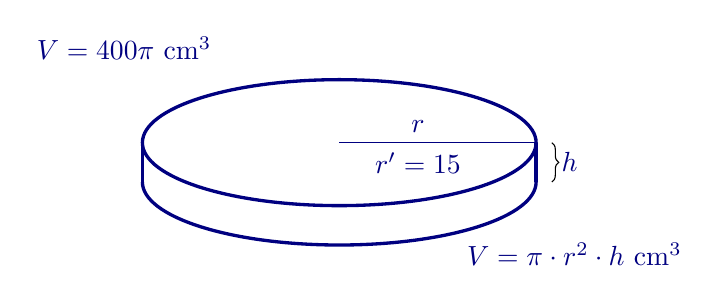
\begin{tikzpicture}
    \draw[penColor,very thick] (0,0) ellipse (2.5 and .8);
    \draw[very thick,penColor] (-2.5,-.5) arc (180:360:2.5 and .8);% bottom
    \draw[penColor] (0,0) -- (2.5,0);
    \draw[penColor,very thick] (-2.5,0) -- (-2.5,-.5);
    \draw[penColor,very thick] (2.5,0) -- (2.5,-.5);
    \node[above,penColor] at (1,0) {$r$};
    \node[below,penColor] at (1,0) {$r' = 15$};
    \draw[decoration={brace,raise=.2cm},decorate,thin] (2.5,0)--(2.5,-.5);
    \node [penColor,right] at (2.7,-.25) {$h$};
    \node [penColor,left] at (-1.5,1.2) {$V = 400\pi$ cm$^3$};
    \node [penColor, right] at (1.5,-1.42) {$V = \pi\cdot r^2 \cdot h$ cm$^3$};
  \end{tikzpicture}
  \end{image}
  Next we need to \textbf{find equations}. We see that we have
  \[
  400\pi = \answer[given]{\pi \cdot r^2 \cdot h},
  \]
  which immediately simplifies to
  \[
  400 = r^2 \cdot h.
  \]
  Since both $r$ and $h$ are functions of time, we now write
  \[
  400 = r(t)^2 \cdot h(t).
  \]
  Now we \textbf{differentiate} both sides of  the equation using implicit
  differentiation, treating all functions as functions of $t$,
  \[
  0 = 2\cdot r(t) \cdot r'(t) \cdot h(t) + r(t)^2 \cdot h'(t).
  \]
  Now we'll \textbf{evaluate} all  the quantities at the moment when $r=20$. 
  But, first, we have to compute $h$ at that moment. Since
  \[
 400 = 20^2 \cdot h, 
  \] it follows that $h=1$, when $r=20$. Now, we are ready to \textbf{solve}.
  
 \[
 0 = 2\cdot 20 \cdot 15 \cdot 1 + 20^2 \cdot \Bigl[\frac{d}{dt}h\Bigr]_{r=20}
  \]
  \begin{align*}
    -2\cdot 20 \cdot 15  &= 20^2 \cdot  \Bigl[\frac{d}{dt}h\Bigr]_{r=20}\\
    \frac{-2\cdot 20 \cdot 15}{20^2}  &=  \Bigl[\frac{d}{dt}h\Bigr]_{r=20}\\
    -1.5  &=  \Bigl[\frac{d}{dt}h\Bigr]_{r=20}
  \end{align*}
  Hence, the thickness of the dough is changing at a rate of $\answer[given]{-1.5}$
  cm/min.
\end{explanation}
\end{example}



\begin{example}
  Consider a melting snowball. We will assume that the rate at which the
  snowball is melting is proportional to its surface area. Show that
  the radius of the snowball is changing at a constant rate.
  
\begin{explanation}
First, we \textbf{introduce the variables} $V$, $r$, and $A$. Let $V$ denote the volume of the snowball, let $r$ denote the radius of the snowball, and  let $A$ be the surface area of the snowball . Then, we \textbf{identify} the given rate $\frac{dV}{dt}$  and the unknown rate $\frac{dr}{dt}$, the rate to be determined. This problem is a bit unusual, because "the given  rate" is not explicitly given. We will deal with this issue below. 
  Next, we \textbf{draw a picture}.
  \begin{image}
    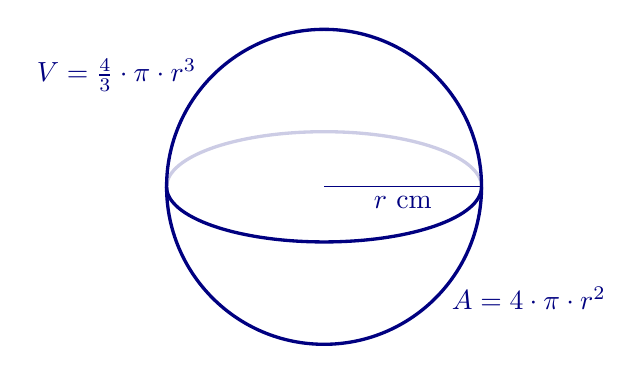
\begin{tikzpicture}
      %\draw[penColor!50!background,very thick] (0,0) ellipse (2 and 1);
      \draw[very thick,penColor!20!background] (2,0) arc (0:180:2 and .7);% top half of ellipse
      \draw [penColor, very thick] (0,0) circle [radius=2];
      \draw[penColor] (0,0) -- (2,0);
      \node [below,penColor] at (1,0) {$r$ cm};
      \draw[very thick,penColor] (-2,0) arc (180:360:2 and .7);% bottom half of ellipse
      \node [penColor,left] at (-1.5,1.42) {$V = \frac{4}{3}\cdot \pi \cdot r^3$};
      \node [penColor, right] at (1.5,-1.42) {$A = 4\cdot \pi \cdot r^2$};
    \end{tikzpicture}
  \end{image}
  Now we need to \textbf{find equations} that relate all relevant variables. The equations we'll use are
  \[
  V = \answer[given]{(4/3) \cdot \pi \cdot r^3} \qquad\text{and}\qquad A = \answer[given]{4\cdot
  \pi \cdot r^2}.
  \]
  Now the key words are ``the rate at which the snowball is melting (the "given" rate) is
  proportional to its surface area.'' From this we have the following
  equation:
  \begin{image}
    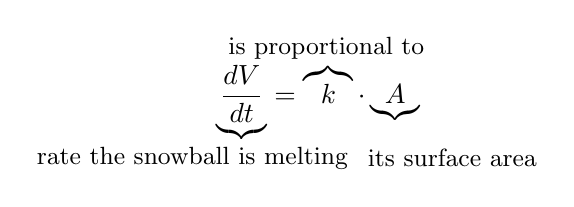
\begin{tikzpicture}
    \node at (0,0) {
      $\underbrace{\frac{dV}{dt}} =  \overbrace{k} \cdot \underbrace{A}$
    };
    \node at (-1.6,-.7) {\small{rate the snowball is melting}};
    \node at (.1,.7) {\small{is proportional to}};
    \node at (1.7,-.7) {\small{its surface area}};
    \end{tikzpicture}
  \end{image}
  We need to compute  $\frac{dV}{dt}$. We know $V = \frac{4}{3}\cdot \pi\cdot
  r^3$. Since $r$ is a function of $t$, we  write 
    \[
  V(t) = \frac{4}{3}\cdot \pi\cdot r(t)^3.
  \]
So
  \[
  \frac{dV}{dt} = 4\cdot \pi\cdot r(t)^2 \cdot \frac{dr}{dt}.
  \]
  We also know that
   \[
 \frac{dV}{dt} = k\cdot A(t).
  \]
  So,
  \[
 4\cdot \pi \cdot r(t)^2 \cdot \frac{dr}{dt} =  k\cdot 4\cdot
  \pi \cdot r(t)^2 .
  \]
 Therefore, we \textbf{solve} for $\frac{dr}{dt}$ and obtain that
  \begin{align*}
\frac{dr}{dt} &=  k.\\
  \end{align*}
  Hence, the radius is changing at a constant rate. Notice, in this example we did not have to evaluate quantities at particular time,  because the unknown rate did not depend on time.
\end{explanation}
\end{example}

\section{Right triangles}

\begin{example}
A road running north to south crosses a road going east to west at the
point $P$.  Cyclist $A$ is riding north along the first road, and
cyclist $B$ is riding east along the second road.  At a particular
time, cyclist $A$ is $3$ kilometers to the north of $P$ and traveling
at $20$ km/hr, while cyclist $B$ is $4$ kilometers to the east of $P$
and traveling at $15$ km/hr.  How fast is the distance between the two
cyclists changing at that time?


\begin{explanation}
First, we \textbf{introduce the variables} $a$, $b$, and $c$. Let $a$ denote the distance of cyclist $A$ from the point $P$, let $b$ denote denote the distance of cyclist $B$ from the point $P$, and  let $c$ denote the distance between the two cyclists. We \textbf{identify} the given rates $\Bigl[\frac{da}{dt}\Bigr]_{a=3, b=4}=20$ km/h, $\Bigl[\frac{db}{dt}\Bigr]_{a=3, b=4}=15$ km/h  and the unknown rate $\Bigl[\frac{dc}{dt}\Bigr]_{a=3, b=4}$. 
Now, we \textbf{draw a picture}.
\begin{image}
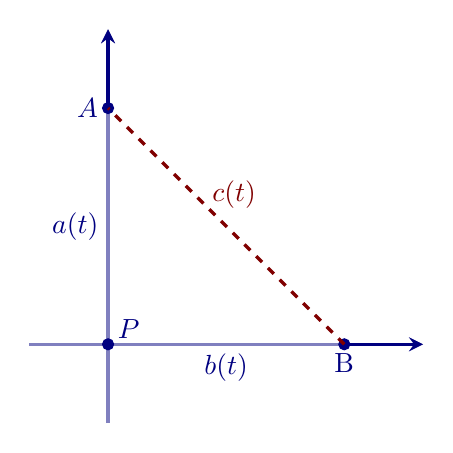
\begin{tikzpicture}
\draw[->,penColor!50!background, very thick] (-1,0) -- (4,0);
\draw[->,penColor!50!background, very thick] (0,-1) -- (0,4);
\draw[->,penColor, very thick] (0,3) -- (0,4);
\draw[->,penColor, very thick] (3,0) -- (4,0);
\draw [penColor, fill] (0,0) circle [radius=.07];
\draw [penColor, fill] (3,0) circle [radius=.07];
\draw [penColor, fill] (0,3) circle [radius=.07];
\draw[dashed,penColor2, very thick] (3,0) -- (0,3);

%\node[penColor,rotate=90,right] at (.5,3) {\scalebox{-2} \Bicycle};
\node[penColor,right] at (0,.2) {$P$};
\node[penColor,left] at (0,1.5) {$a(t)$ };
\node[penColor,left] at (-.005,3) {$A$ };
\node[penColor,below] at (1.5,0) {$b(t)$ };
\node[penColor,below] at (3,0) {B};
\node[penColor2,above] at (1.6,1.6) {$c(t)$};
%\node[penColor,right,above] at (3.5,0) {\scalebox{-2}[2] \Bicycle};
\end{tikzpicture}
\end{image}
We \textbf{find equations} relating variables $a$, $b$, and $c$.  By the Pythagorean Theorem,
\[
c(t)^2=a(t)^2+b(t)^2.
\] 
Now we  \textbf{differentiate} both sides of  the equation. 
\[
2c(t)c'(t)=2a(t)a'(t)+2b(t)b'(t).
\]
Next, we will \textbf{evaluate} all the quantities in this equation at the time when $a=3$ and $b=4$.
We see that we $c$ needs to be evaluated at that time, too. In order to do that, 
let's draw and label the picture at the time when $a=3$ and $b=4$.
\begin{image}
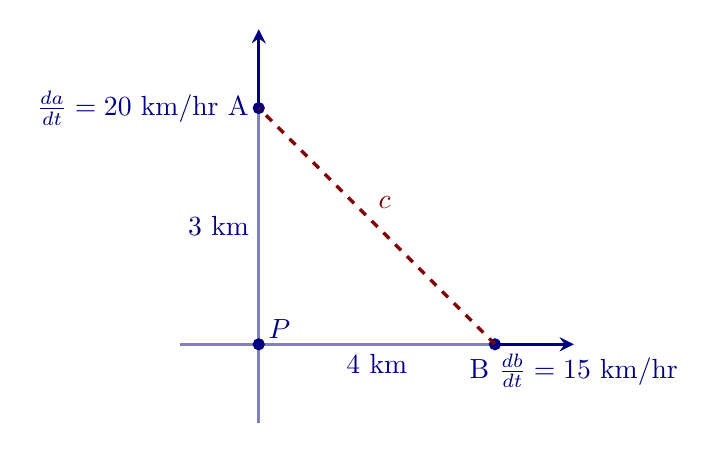
\begin{tikzpicture}
\draw[->,penColor!50!background, very thick] (-1,0) -- (4,0);
\draw[->,penColor!50!background, very thick] (0,-1) -- (0,4);
\draw[->,penColor, very thick] (0,3) -- (0,4);
\draw[->,penColor, very thick] (3,0) -- (4,0);
\draw [penColor, fill] (0,0) circle [radius=.07];
\draw [penColor, fill] (3,0) circle [radius=.07];
\draw [penColor, fill] (0,3) circle [radius=.07];
\draw[dashed,penColor2, very thick] (3,0) -- (0,3);

%\node[penColor,rotate=90,right] at (.5,3) {\scalebox{-2} \Bicycle};
\node[penColor,right] at (0,.2) {$P$};
\node[penColor,left] at (-.005,3) {$\frac{da}{dt} = 20$ km/hr A};
\node[penColor,left] at (0,1.5) {$3$ km};
\node[penColor,below] at (1.5,0) {$4$ km};
\node[penColor,below] at (4,0) {B  $\frac{db}{dt}= 15$ km/hr };
\node[penColor2,above] at (1.6,1.6) {$c$};
%\node[penColor,right,above] at (3.5,0) {\scalebox{-2}[2] \Bicycle};
\end{tikzpicture}
\end{image}
By the the Pythagorean Theorem and the picture above, it follows that
\[
c = \answer[given]{5}  km
\]
Now we  \textbf{evaluate} all the quantities at the time when $a=3$ and $b=4$, and get 
\[
2\cdot 5 \cdot \Bigl[\frac{dc}{dt}\Bigr]_{a=3, b=4} = 2 \cdot 3\cdot 20 + 2 \cdot 4 \cdot 15.
\]
\textbf{Solving} for $\Bigl[\frac{dc}{dt}\Bigr]_{a=3, b=4}$ we find that

 $\Bigl[\frac{dc}{dt}\Bigr]_{a=3, b=4} = \answer[given]{24}$ km/hr.\\
\end{explanation}
\end{example}


\begin{example}
A plane is flying at an altitude of $3$ miles directly away from you at $500$ mph 
.  How fast is the plane's distance from you increasing at
the moment when the plane is flying over a point on the ground $4$
miles from you?


\begin{explanation}
 First, we \textbf{introduce variables} $p$, the distance the plane has traveled after the moment when it flew right above you, and $s$, the distance between you and the plane. 
The given rate is $\frac{dp}{dt}=500$ mph and the unknown (related) rate is $\Bigl [\frac{ds}{dt}\Bigr]_{p=4}$.
Next, we \textbf{draw a picture}.
\begin{image}
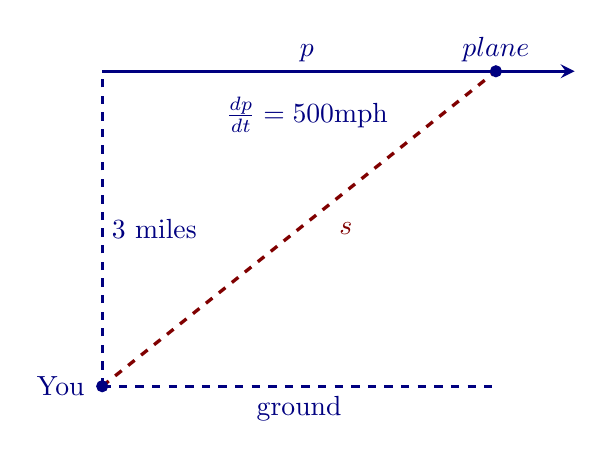
\begin{tikzpicture}
\draw[penColor2, dashed, very thick] (0,0) -- (5,4);
%\draw[penColor, dashed, very thick] (0,0) -- (0,4);
\draw[penColor, dashed, very thick] (0,0) -- (0,4);
\draw[penColor, dashed, very thick] (0,0) -- (5,0);
\draw[->,penColor, very thick] (0,4) -- (6,4);
\draw [penColor, fill] (5,4) circle [radius=.07];
%\node [left,penColor] at (0,0) {\scalebox{3} \Ladiesroom};
%\node [right,penColor] at (6,4) {\scalebox{3}{\ding{40}}};
\node [right,penColor] at (0,2) {$3$ miles};
\node [above,penColor] at (2.6,4) {$p$ };
\node [above,penColor] at (5,4) {$plane$ };
\node [above,penColor] at (2.6,3.1) {$\frac{dp}{dt}=500$mph};
\node [below,penColor] at (2.5,0) {ground};
\node [left,penColor2] at (3.3,2) {$s$ };
\draw [penColor, fill] (0,0) circle [radius=.07];
\node [left,penColor] at (-.1,0) {You};
\end{tikzpicture}
\end{image}
Next we \textbf{find equations} relating the variables $p$ and $s$. By the Pythagorean Theorem
we know that
\[
p^2+3^2=s^2.
\] 
Since  $p$ and $s$ are functions of time, we now
\textbf{differentiate} both sides of the equation 
\[
2\cdot p(t)\cdot p'(t)  = 2\cdot s(t) \cdot s'(t).
\] 
Next  we \textbf{evaluate} all the quantities at the moment when $p=4$ miles. This implies that $s$ has to be evaluated at time when $p=4$. In order to do that,
 let's draw the picture at the moment when $p=4$ mi.
\begin{image}
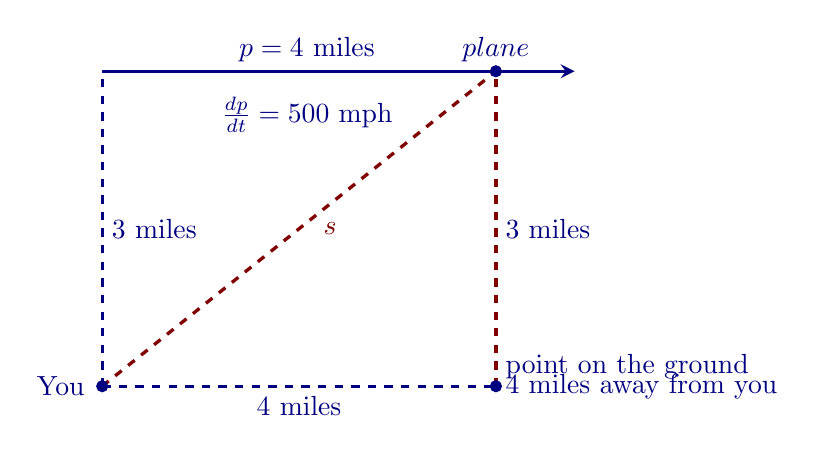
\begin{tikzpicture}
\draw[penColor2, dashed, very thick] (0,0) -- (5,4);
\draw[penColor2, dashed, very thick] (5,0) -- (5,4);
%\draw[penColor, dashed, very thick] (0,0) -- (0,4);
\draw[penColor, dashed, very thick] (0,0) -- (0,4);
\draw[penColor, dashed, very thick] (0,0) -- (5,0);
\draw[->,penColor, very thick] (0,4) -- (6,4);
\draw [penColor, fill] (5,4) circle [radius=.07];
\draw [penColor, fill] (5,0) circle [radius=.07];
%\node [left,penColor] at (0,0) {\scalebox{3} \Ladiesroom};
%\node [right,penColor] at (6,4) {\scalebox{3}{\ding{40}}};
\node [right,penColor] at (0,2) {$3$ miles};
\node [right,penColor] at (5,2) {$3$ miles};
\node [right,penColor] at (5,0.25) {point on the ground};
\node [right,penColor] at (5,0) {4 miles away from you };
\node [above,penColor] at (2.6,3.1) {$\frac{dp}{dt} = 500$ mph};
\node [above,penColor] at (2.6,4) {$p=4$ miles};
\node [above,penColor] at (5,4) {$plane$ };
\node [below,penColor] at (2.5,0) {$4$ miles};
\node [left,penColor2] at (3.1,2) {$s$ };
\draw [penColor, fill] (0,0) circle [radius=.07];
\node [left,penColor] at (-.1,0) {You};
\end{tikzpicture}
\end{image}

By applying the Pythagorean Theorem, we find that $4^2+3^2=s^2$, so
$s=\answer[given]{5}$.  Putting together all the information we get
\[
2(4)(500)=2(5)\Bigl[\frac{ds}{dt}\Bigr]_{p=4} .
\]
Finally, we \textbf{solve}:  $\Bigl[\frac{ds}{dt}\Bigr]_{p=4}=\answer[given]{400}$ mph.
\end{explanation}
\end{example}


\section{Angular rates}

\author{Nela Lakos}
\begin{example}
A plane is flying at an altitude of $3$ miles directly away from you at $500$ mph 
.  Let  $\theta$ be the \textbf{angle of elevation} of the plane, i.e., the angle between the ground and your line of  sight to the plane.
How fast is the angle $\theta$  decreasing at
the moment when the plane is flying over a point on the ground $4$
miles from you?


\begin{explanation}
 First, we \textbf{introduce a variable} $p$, the distance the plane has traveled after the moment when it flew right above you. 
 So, the given rate is $\frac{dp}{dt}=500$ mph and the unknown (related) rate is $\Bigl [\frac{d\theta}{dt}\Bigr]_{p=4}$.
  This rate should be measured in rad/s.
  Therefore, we have to convert the units of the given rate, mph, into mi/s:
    $\frac{dp}{dt}=500$mph$=\frac{500}{60\cdot60}$ mi/s. \\
Next, we \textbf{draw a picture}.
\begin{image}
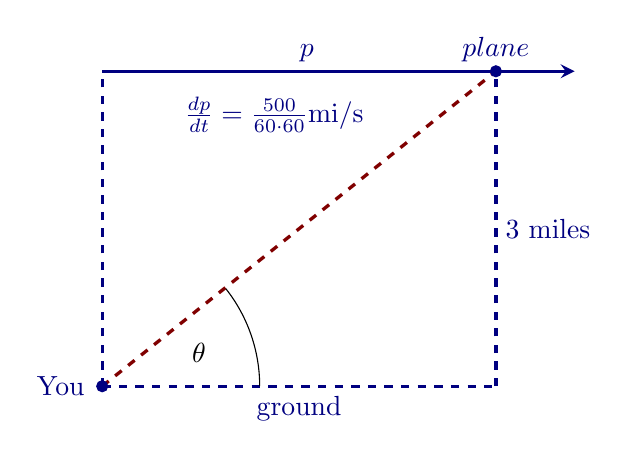
\begin{tikzpicture}
\draw[penColor2, dashed, very thick] (0,0) -- (5,4);
%\draw[penColor, dashed, very thick] (0,0) -- (0,4);
\draw[penColor, dashed, very thick] (0,0) -- (0,4);
\draw[penColor, dashed, very thick] (5,0) -- (5,4);
\draw[penColor, dashed, very thick] (0,0) -- (5,0);
\draw[->,penColor, very thick] (0,4) -- (6,4);
\draw [penColor, fill] (5,4) circle [radius=.07];
\coordinate (A) at (3.3,2.6);
        \coordinate (B) at (0,0);
        \coordinate (C) at (4,0);
\tkzMarkAngle[size=2cm,thin](C,B,A)
        \tkzLabelAngle[pos = 1.3](C,B,A){$\theta$}
%\node [left,penColor] at (0,0) {\scalebox{3} \Ladiesroom};
%\node [right,penColor] at (6,4) {\scalebox{3}{\ding{40}}};
\node [right,penColor] at (5,2) {$3$ miles};
\node [above,penColor] at (2.6,4) {$p$ };
\node [above,penColor] at (5,4) {$plane$ };
\node [above,penColor] at (2.18,3.1) {$\frac{dp}{dt}=\frac{500}{60\cdot60}$mi/s};
\node [below,penColor] at (2.5,0) {ground};
\draw [penColor, fill] (0,0) circle [radius=.07];
\node [left,penColor] at (-.1,0) {You};
\end{tikzpicture}
\end{image}
Now we  \textbf{find an equation} relating variables $p$ and $\theta$.
From the picture we can see that
\[
\tan{\theta}=\frac{3}{p}.
\] 
Since  $p$ and $\theta$ are both functions of time, we now
\textbf{differentiate} both sides of the equation. We write
\[
\sec^{2}{\theta}\cdot\theta'  = -\frac{3}{p^2}\cdot p'.
\] 
The above equation holds over some interval of time. In particular, it is true when $p=4$.
Now, we draw and label the picture at the moment when $p=4$ mi.
\begin{image}
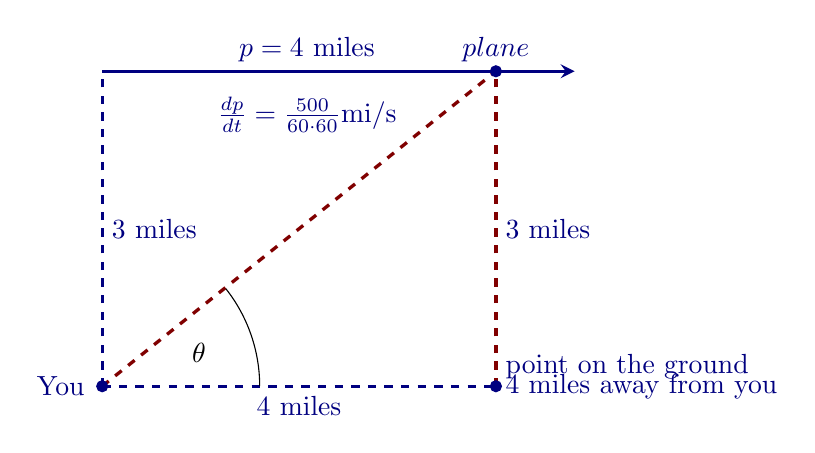
\begin{tikzpicture}
\draw[penColor2, dashed, very thick] (0,0) -- (5,4);
\draw[penColor2, dashed, very thick] (5,0) -- (5,4);
%\draw[penColor, dashed, very thick] (0,0) -- (0,4);
\draw[penColor, dashed, very thick] (0,0) -- (0,4);
\draw[penColor, dashed, very thick] (0,0) -- (5,0);
\draw[->,penColor, very thick] (0,4) -- (6,4);
\draw [penColor, fill] (5,4) circle [radius=.07];
\draw [penColor, fill] (5,0) circle [radius=.07];
\coordinate (A) at (3.3,2.6);
        \coordinate (B) at (0,0);
        \coordinate (C) at (4,0);
\tkzMarkAngle[size=2cm,thin](C,B,A)
        \tkzLabelAngle[pos = 1.3](C,B,A){$\theta$}
%\node [left,penColor] at (0,0) {\scalebox{3} \Ladiesroom};
%\node [right,penColor] at (6,4) {\scalebox{3}{\ding{40}}};
\node [right,penColor] at (0,2) {$3$ miles};
\node [right,penColor] at (5,2) {$3$ miles};
\node [right,penColor] at (5,0.25) {point on the ground};
\node [right,penColor] at (5,0) {4 miles away from you };
\node [above,penColor] at (2.6,3.1) {$\frac{dp}{dt} =\frac{500}{60\cdot60}$mi/s};
\node [above,penColor] at (2.6,4) {$p=4$ miles};
\node [above,penColor] at (5,4) {$plane$ };
\node [below,penColor] at (2.5,0) {$4$ miles};
\draw [penColor, fill] (0,0) circle [radius=.07];
\node [left,penColor] at (-.1,0) {You};
\end{tikzpicture}
\end{image}

We now \textbf{evaluate} all the quantities at the moment when $p=4$. First, we have to compute $\sec^{2}{\theta}$ at that time.
We will remind ourselves of the trig identity
\[
\sec^2{\theta}=1+\tan^2{\theta}.
\] 
So,
\[
\Big[\sec^2{\theta}\Bigr]_{p=4}=1+\Bigr(\frac{3}{4}\Bigl)^2=\frac{25}{16}.
\] 
Now, by substituting all the known values into the equation above, we get
\[
\frac{25}{16}\cdot\Bigl [\frac{d\theta}{dt}\Bigr]_{p=4} = -\frac{3}{16}\cdot \frac{500}{60\cdot60}.
\] 
We \textbf{solve} for $\Bigl [\frac{d\theta}{dt}\Bigr]_{p=4}$ and get that
\[
\Bigl [\frac{d\theta}{dt}\Bigr]_{p=4} = -\frac{1}{60}  rad/s.
\] 
\end{explanation}
\end{example}

\section{Similar triangles}

\begin{example}
  It is night. Someone who is $6$ feet tall is walking away from a
  street light at a rate of $3$ feet per second.  The street light is
  $15$ feet tall.  The person casts a shadow on the ground in front of
  them. How fast is the length of the shadow growing when the person
  is $7$ feet from the street light?

  \begin{explanation}
  First, we \textbf{introduce two variables}, $p$ and $s$. Let $p$ be the distance from the person to the lamp, and let $s$ be the length of the shadow.
  So, the given rate is $\frac{dp}{dt}=3$ ft/s and the unknown (related) rate is $\Bigl[\frac{ds}{dt}\Bigr]_{p=7}$.
    Then, we \textbf{draw a picture}.
    \begin{image}
      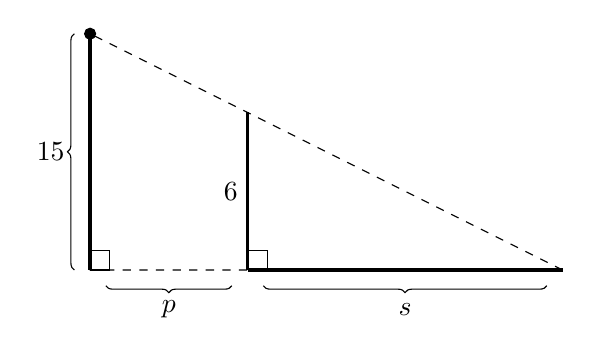
\begin{tikzpicture}
        \coordinate (A) at (6,2);
        \coordinate (B) at (0,5);
        \coordinate (C) at (0,2);
        \coordinate (D) at (2,2);
        \coordinate (E) at (2,4);
        \tkzMarkRightAngle(A,C,B)
        \tkzMarkRightAngle(A,D,E)
        \tkzDefMidPoint(A,B) \tkzGetPoint{a}
        \tkzDefMidPoint(A,C) \tkzGetPoint{b}
        \tkzDefMidPoint(D,C) \tkzGetPoint{x}
        \draw[decoration={brace,mirror,raise=.2cm},decorate,thin] (.2,2)--(1.8,2);
        \draw[decoration={brace,mirror,raise=.2cm},decorate,thin] (2.2,2)--(5.8,2);
        \draw[decoration={brace,raise=.2cm},decorate,thin] (0,2)--(0,5);
        \draw[dashed] (A)--(B)--(C)--cycle;
        \draw[very thick] (D)--(E);
        \draw[very thick] (D)--(A);
        \draw[very thick] (B)--(C);
        \node[left] at (2,3) {$6$};
        \node at (1,2-.5) {$p$};
        \node at (4,2-.5) {$s$};
        \node at (0-.5,3.5) {$15$};
        \draw [fill] (0,5) circle [radius=.07];
      \end{tikzpicture}
    \end{image}

    Now we \textbf{find equations} that relate the variables $p$ and $s$. We use the fact that we
    have similar triangles to write:
    \begin{align*}
      \frac{s+p}{\answer[given]{15}} &= \frac{s}{\answer[given]{6}},\\
      6\cdot s + 6 \cdot p &= 15\cdot s,\\
      6\cdot p &=9\cdot s,\\
      2\cdot p &=3 \cdot s. 
    \end{align*}
    Since, $p$ and $s$ are both functions of time, we 
  \textbf{differentiate} both sides of the equation above. We  use
    implicit differentiation and write
        \[
    2\cdot p'(t) =3 \cdot s'(t)
    \]
    At this point we \textbf{evaluate} all the quantities at time when $p=7$ ft 
    \[
    2\cdot 3 = 3 \cdot \Bigl[\frac{ds}{dt}\Bigr]_{p=7}.
    \]
    Now we \textbf{solve} for  $\Bigl[\frac{ds}{dt}\Bigr]_{p=7} $ and get that
     $\Bigl[\frac{ds}{dt}\Bigr]_{p=7} = \answer[given]{2}$, 
      meaning the shadow is growing
    at a rate of $2$ feet per second when the person is $7$ ft from the lamp.\\
  \end{explanation}
\end{example}


\begin{example}
Water is poured into a conical container at the rate of 10
cm${}^3$/s.  The cone points directly down, and it has a height of
30 cm and a base radius of 10 cm.  How fast is the water level rising
when the water is 4 cm deep?

\begin{explanation}
First, we \textbf{introduce several variables}, $V$, $r$, and $h$. Let $V$ denote the volume of the water in the container, let $r$ denote the radius of the circlular surface of the water, and  let $h$ be the depth of the water in the container. The given rate is $\frac{dV}{dt}=10$ $cm^3/s$, and the unknown rate is $\Bigl[\frac{dh}{dt}\Bigr]_{h=4}$.
    Now, we \textbf{draw a picture}.
\begin{image}
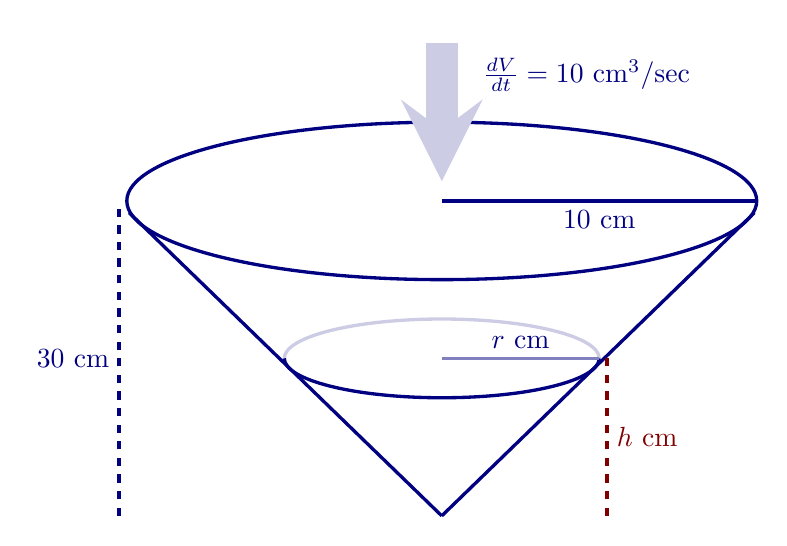
\begin{tikzpicture}
\draw[penColor,very thick] (0,4) ellipse (4 and 1);
\draw[very thick,penColor!20!background] (2,2) arc (0:180:2 and .5);% top half of ellipse
\draw[very thick,penColor] (-2,2) arc (180:360:2 and .5);% bottom half of ellipse
\draw[penColor, very thick] (3.97,3.85) -- (0,0);
\draw[penColor, very thick] (-3.97,3.85) -- (0,0);
\draw[penColor, very thick] (0,4) -- (4,4);
\draw[penColor!50!background, very thick] (0,2) -- (2,2);
\draw[->,line width=0.4cm, penColor!20!background] (0,6) -- (0,4.25);
\draw[dashed, penColor2, very thick] (2.1,0) -- (2.1,2);
\draw[dashed, penColor, very thick] (-4.1,0) -- (-4.1,4);
\node[right, penColor] at (.4,5.6) {$\dd[V]{t} = 10$ cm$^3$/sec};
\node[below, penColor] at (2,4) {$10$ cm};
\node[above, penColor] at (1,2) {$r$ cm};
\node[right, penColor2] at (2.1,1) {$h$ cm};
\node[left, penColor] at (-4.1,2) {$30$ cm};
\end{tikzpicture}
\end{image}
Note, no attempt was made to draw this picture to scale, rather we
want all of the relevant information to be available to the
mathematician.

Now we \textbf{find equations} that relate all the variables. Notice that water in the container assumes the shape of the container. In this example, the shape is a cone. Therefore, we use the formula for the volume of
a cone 
\[
V = \frac{\pi}{3} r^2 h.
\]
Let's draw a cross section of the cone.
\begin{image}
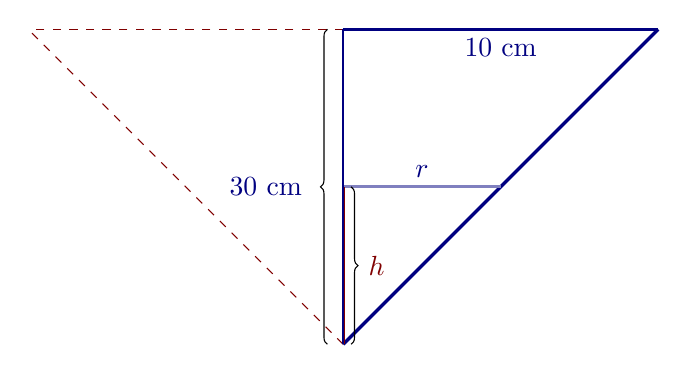
\begin{tikzpicture}
\draw[penColor, very thick] (4,4) -- (0,0);
\draw[penColor, very thick] (0,4) -- (4,4);
\draw[penColor2, thick] (0,2) -- (0,0);
\draw[penColor!50!background, very thick] (0,2) -- (2,2);
\draw[dashed, penColor2,  thin] (0,0) -- (-4,4);
\draw[dashed, penColor2, thin] (0,4) -- (-4,4);
\draw[ penColor2, very thick] (0,0) -- (0,2);
\draw[ penColor,thick] (0,0) -- (0,4);
  \draw[decoration={brace,raise=.2cm},decorate,thin] (0,0)--(0,4);
    \draw[decoration={brace, mirror,raise=.1cm},decorate,thin] (0,0)--(0,2);
\node[below, penColor] at (2,4) {$10$ cm};
\node[above, penColor] at (1,2) {$r$ };
\node[right, penColor2] at (0.2,1) {$h$ };
\node[left, penColor] at (-0.4,2) {$30$ cm};
\end{tikzpicture}
\end{image}
Notice a big right triangle and  a smaller right triangle inside the big one.
These two right triangles are similar, because their corresponding angles are equal.
Since the ratios of corresponding sides in similar triangles are equal, we get
\[
\frac{r}{h}=\frac{10}{30} \qquad\text{so}\qquad r=\answer[given]{h/3}.
\]  
Now we  \textbf{differentiate} both sides of each equation using
implicit differentiation.

\[
\dd[V]{t} = \frac{\pi}{3}\left(2rh \dd[r]{t} + r^2 \dd[h]{t}\right)
\qquad\text{and}\qquad \dd[r]{t} = \frac{1}{3}\cdot \dd[h]{t}.
\]
These two equations hold over some time interval. In particular, the equations are true at time when $h=4$ cm. 
Now we \textbf{evaluate} all the quantities at that time. We plug in $\dd[V]{t} =
\answer[given]{10}$, $r = \answer[given]{4/3}$, $\dd[r]{t} = \frac{1}{3}\cdot \Bigl[\dd[h]{t}\Bigr]_{h=4}$ and
$h=\answer[given]{4}$.
\begin{align*}
10 &= \frac{\pi}{3}\left(2\cdot \frac{4}{3}\cdot 4 \cdot\frac{1}{3}\cdot\Bigl[\dd[h]{t}\Bigr]_{h=4} + \left(\frac{4}{3}\right)^2 \Bigl[\dd[h]{t}\Bigr]_{h=4}\right)\\Now,\hspace{0.025in}\textbf{solve.}\\
10 &= \frac{\pi}{3}\left(\frac{32}{9}\Bigl[\dd[h]{t}\Bigr]_{h=4} + \frac{16}{9} \Bigl[\dd[h]{t}\Bigr]_{h=4}\right)\\ 
10 &= \frac{16\pi}{9}\Bigl[\dd[h]{t}\Bigr]_{h=4}\\
\frac{90}{16\pi} &= \Bigl[\dd[h]{t}\Bigr]_{h=4}.
\end{align*}
Thus, $\Bigl[\dd[h]{t}\Bigr]_{h=4}=\answer[given]{\frac{90}{16\pi}}$ cm/s.
\end{explanation}
\end{example}
\end{document}



